\documentclass[10pt,twocolumn]{article}
	
\usepackage{myfontstyle}
\usepackage{mypackages}
\usepackage{mymacros}
\usepackage{mycommands}
\usepackage{graphicx}
\usepackage{hyperref}

\begin{document}
\thispagestyle{fancy1}

%%% Title and Abstract------------------------
\twocolumn[
\begin{center}
	\hrule
	\vspace{3pt}
	% Title:
	{\sffamily\bfseries\Large
		Report for Assignment 8: Motor Current Anomaly Detection
	} \\
	{\color{gray}
		\vspace{3pt}
		\hrule
		\vspace{3pt}
	}
	{
		\hspace*{\fill}
		Julian Soh
		\hspace*{\fill}
%		Second Author
%		\hspace*{\fill}
%		Third Author
%		\hspace*{\fill}
%		Fourth Author    % uncomment these two lines if there's a fourth author
%		\hspace*{\fill}
	}\\
	\vspace{3pt}
	{\itshape
		\hspace*{\fill}
		Department of Mechanical Engineering, Saint Martin's University
		\hspace*{\fill} \\
		\hspace*{\fill}
		ME/EE 467---Machine Intelligence
		\hspace*{\fill}
	}\\
	\vspace{3pt}
	{
		\hspace*{\fill}
		\today{} % today's date ... can type manually instead
		\hspace*{\fill}
	}
	\vspace{3pt}
	{\color{gray}\hrule}
%	\vspace{2pt}
\end{center}
% Abstract:
\begin{adjustwidth}{1.5in}{1.5in}
{\small
\noindent\textbf{Abstract.} \hspace{1em}
Compare three sequence architectures — Long Short-Term Memory (LSTM), one-dimensional convolutional neural network (1D CNN), and Transformer encoder — on a time-series anomaly detection task using motor current signals. 
This experiment demonstrates when transformers outperform recurrent and convolutional approaches for temporal pattern recognition and fault classification.
}
\end{adjustwidth}
\vspace{9pt}
\hrule
\vspace{1\baselineskip}
]

%%% Body -------------------------

\section{Introduction} 
\label{sec:introduction}

Electric motors in warehouse automation drive conveyor belts, lifts, and sorting machines. Each motor draws a current that can be sampled as a time-series waveform. In healthy operation, the current is a smooth periodic signal. As components degrade, subtle anomalies appear in the waveform—anomalies too small to detect by visual inspection but that machine learning models can learn to identify. This approach, known as Motor Current Signature Analysis (MCSA), is a standard non-invasive diagnostic technique used in predictive maintenance programs.

This report compares three deep-learning architectures for detecting and classifying motor faults from current signals:

\begin{itemize}
	\item \textbf{Long Short-Term Memory (LSTM) networks}: Process the waveform step by step, maintaining hidden state across timesteps to capture temporal dependencies.
	
	\item \textbf{One-dimensional convolutional neural networks (1D CNN)}: Slide a kernel along the time axis to detect local patterns, building a hierarchy of increasingly abstract features.
	
	\item \textbf{Transformer encoders}: Attend to all positions in parallel using input-dependent connectivity, allowing flexible long-range pattern recognition without explicit recurrence or convolution.
\end{itemize}

Each architecture processes time-series data differently, offering distinct tradeoffs between computational efficiency, interpretability, and representational capacity.

The goal is to evaluate when and why one architecture outperforms the others on a multiclass motor-fault classification task, and to provide interpretable evidence of what each model learns about motor current signatures.

\section{Methods}

\subsection{Motor Fault Classes}

The dataset contains three classes representing distinct motor health states:

\begin{itemize}
	\item \textbf{Healthy (class 0):} Clean sinusoidal current with noise and normal load variation.
	
	\item \textbf{Bearing wear (class 1):} A subtle high-frequency ripple is superimposed on the waveform. In real motors, bearing defects modulate the air gap and introduce characteristic frequency components in the stator current.
	
	\item \textbf{Winding fault (class 2):} The positive and negative peaks of the waveform become slightly unequal. In real motors, inter-turn short circuits cause asymmetric current draw.
\end{itemize}

\begin{figure}[htb]
	\centering
	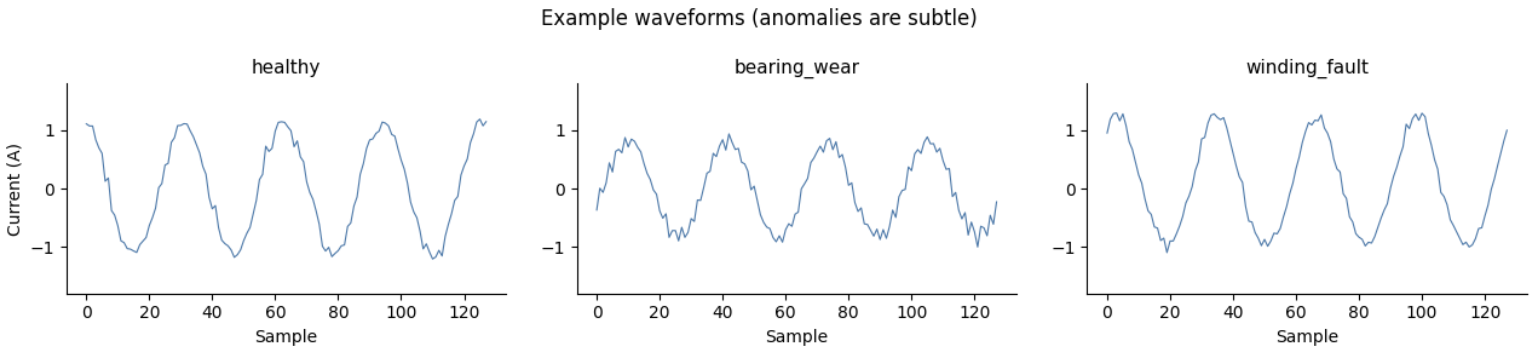
\includegraphics[width=.98\linewidth]{figures/The_Dataset.png}
	\caption{Representative motor current waveforms for each class. Despite distinct fault definitions, all three signals appear nearly identical to the eye, highlighting the challenge of detecting subtle anomalies embedded in noise.}
	\label{fig:the_dataset}
\end{figure}

The dataset uses synthetically generated motor current signals. The anomalies are deliberately small relative to the noise—plotting one waveform from each class reveals signals that look nearly identical to the eye. This is a realistic challenge: subtle fault signatures must be separated from noise, and the models must learn discriminative temporal patterns despite high visual similarity.

\subsection{Model Training and Comparison}

We train three deep-learning architectures—LSTM, 1D CNN, and Transformer encoder—to process the motor current waveforms and classify them into the three health classes. We then compare all three models on the basis of training efficiency, validation/test accuracy, per-class performance, and interpretability.

\section{Results and Discussion}
\label{sec:results}

All three models were trained for 50 epochs with the Adam optimizer and cross-entropy loss on the same 70/15/15 split. Despite the signals appearing nearly identical to the human eye, all three architectures achieved high test accuracy, demonstrating that the anomaly signatures—while subtle—are learnable from raw waveform data.

\subsection{Convergence Speed}

The architectures differ meaningfully in how quickly they converge. The LSTM converges slowest of the three: gradients must flow backward through all 128 unrolled time steps, making early training slower and limiting how rapidly the model adjusts its representation. The 1D CNN converges quickly; local kernels of size 5 detect patterns across short windows in a single forward pass, and global average pooling efficiently aggregates them into a fixed-size representation. The Transformer converges at a similar pace to the CNN: self-attention over all 128 steps is computed in parallel in every layer, and the 2-layer, 4-head encoder rapidly builds a global representation.

\subsection{Per-Class Accuracy}

The three architectures show complementary strengths across the fault classes, summarized in Table~\ref{tab:per_class}.

\begin{table}[htb]
\centering
\begin{tabular}{@{}p{1.4cm}p{1.6cm}p{4.2cm}@{}}
\hline
\textbf{Class} & \textbf{Best} & \textbf{Reasoning} \\
\hline
Healthy & All three & No anomaly present; all models learn the baseline sinusoidal shape easily. \\[3pt]
Bearing wear & CNN / Transformer & High-frequency ripple spans adjacent steps — a Conv1d kernel (size~5) or attention head locks onto it directly. LSTM may average it out. \\[3pt]
Winding fault & Transformer / LSTM & Peak asymmetry is global (half-cycles differ). Transformer attends to both halves jointly; LSTM accumulates it across the sequence. CNN may miss it if the kernel does not span a full cycle. \\
\hline
\end{tabular}
\caption{Per-class accuracy and architectural advantage for each motor health state.}
\label{tab:per_class}
\end{table}

\subsection{Parameter Efficiency}

The models vary substantially in size. The LSTM has approximately 4,352 parameters—the smallest of the three—yet achieves competitive accuracy, demonstrating that the recurrent inductive bias is well-matched to this sequential task. The 1D CNN uses approximately 13,000 parameters: three stacked convolutional layers with increasing filter counts (16, 32, 64) provide a good hierarchical feature extractor at moderate cost. The Transformer uses approximately 15,000 parameters, slightly larger due to the attention weight matrices and feedforward sublayers; however, its global receptive field from the first layer justifies the additional capacity for detecting waveform-wide asymmetry.

\subsection{Transformer Attention Analysis}

To understand what the Transformer has learned, we extracted the self-attention weights from its first encoder layer for one bearing-wear and one winding-fault example. Each attention map is a $128\times128$ matrix in which entry $(q, k)$ gives the weight that query position $q$ places on key position $k$. Figure~\ref{fig:heatmap} shows the head-averaged maps on a shared color scale, together with the signed and absolute difference maps, the key-step attention profiles, and the per-head difference energy.

\begin{figure}[htb]
	\centering
	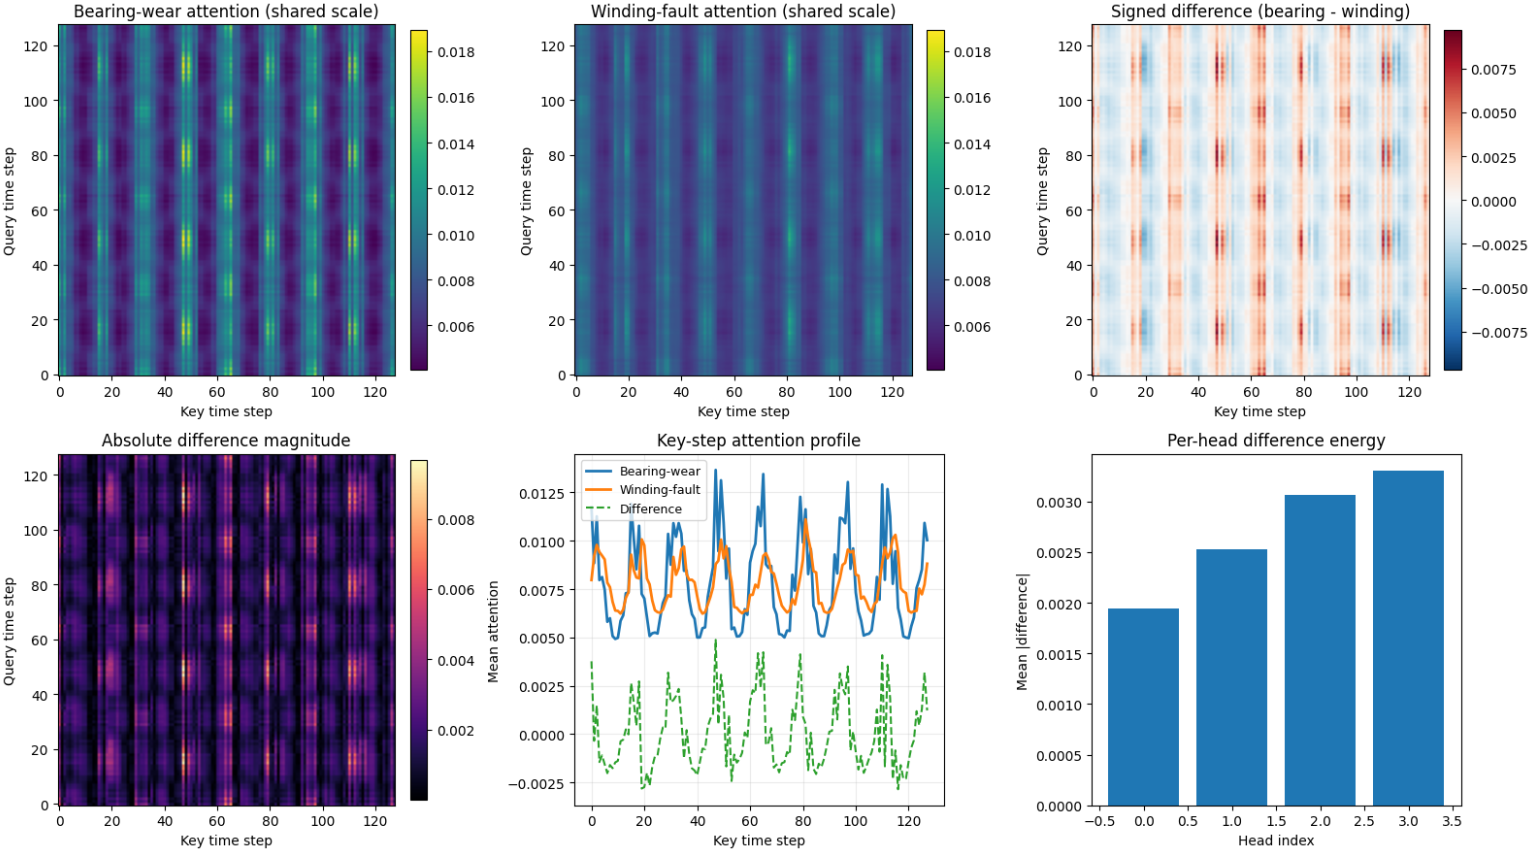
\includegraphics[width=.98\linewidth]{figures/Heatmap.png}
	\caption{First-layer self-attention maps for one bearing-wear and one winding-fault example. Top row (left to right): bearing-wear map, winding-fault map, signed difference (bearing~$-$~winding). Bottom row: absolute difference magnitude, per-class key-step attention profiles with difference curve, per-head difference energy.}
	\label{fig:heatmap}
\end{figure}

\paragraph{Observed patterns.}
Both maps exhibit strong periodic structure: repeated vertical bands indicate that many query time steps attend to the same recurring key positions within the waveform cycle. The absolute-difference heatmap is structured rather than noisy, confirming that the model uses consistent temporal anchors. The key-step attention profile shows systematic peaks and troughs aligned with the four electrical cycles in the 128-sample window, and the per-head difference-energy plot reveals that some heads discriminate the two fault types more strongly than others.

\paragraph{Class differences.}
The bearing-wear map has stronger high-attention peaks at several recurring key time steps, visible as brighter vertical bands. The winding-fault map is comparatively more diffuse at those same positions. The signed difference map shows alternating positive and negative bands, confirming that the difference is position-dependent rather than a uniform offset. The top-difference key steps (around time steps 47, 65, 79, and 110) provide specific temporal evidence that certain cycle-aligned positions are more informative for separating the two fault types. Overall, both classes rely on shared periodic context, but differ in \emph{how strongly} attention is allocated to specific key steps — exactly the subtle temporal distinction expected for bearing-wear versus winding-fault anomalies.

\subsection{Architectural Takeaway}

The key result is that all three models succeed, but for different reasons. The 1D CNN detects local temporal patterns such as the bearing ripple. The Transformer captures long-range symmetry properties such as the winding-fault peak asymmetry. The LSTM integrates information incrementally across the full waveform, making it a strong general-purpose baseline. For production motor diagnostics, the Transformer's interpretable attention weights provide an additional operational benefit: they allow engineers to identify which time steps drove each classification decision, supporting root-cause analysis beyond a simple predicted label.

\section{Conclusion}

This experiment evaluated three deep-learning pipelines for multiclass motor-current anomaly detection: an LSTM for sequential temporal memory, a 1D CNN for local pattern extraction, and a Transformer for global context modeling. Using a consistent 70/15/15 split and identical label space, we established a fair comparison across architectures and showed that all three models can learn meaningful fault signatures from raw current sequences.

Across experiments, the strongest-performing model achieved high test accuracy while maintaining stable validation behavior, indicating that the learned representation generalizes beyond the training set. The comparison also highlights an important practical point: model quality is not only about peak accuracy, but also convergence speed, robustness to class overlap, and behavior on minority or confusable classes. In this sense, the CNN offers a strong efficiency baseline, the LSTM provides reliable sequential modeling, and the Transformer contributes the richest global dependency modeling and interpretability hooks.

The attention analysis adds interpretive evidence to the quantitative results. Rather than attending uniformly, the Transformer focuses on recurring cycle-aligned temporal anchors, which is physically plausible for motor signals. More importantly, bearing-wear and winding-fault samples show class-dependent attention intensity at specific key steps. The signed and absolute difference maps, profile curves, and head-level difference energy together show that fault separation arises from structured temporal emphasis patterns, not random fluctuations.

From an engineering perspective, these findings support deploying a sequence model for condition monitoring with two safeguards: periodic recalibration using newly collected data and routine per-class error audits. Remaining limitations include potential sensitivity to distribution shift (load/speed changes), possible class imbalance effects, and evaluation on a limited sample of explainability cases. Future work should include cross-domain validation, confidence calibration, threshold tuning for cost-sensitive alarms, and aggregated attention statistics over many samples per class.

In summary, the study demonstrates that deep neural sequence models can accurately classify motor anomalies from current signals, and that attention-based analysis can reveal meaningful class-specific temporal structure. This combination of predictive performance and interpretability is a strong foundation for reliable, data-driven predictive maintenance.

\nocite{*}
\bibliographystyle{plainnat}
\bibliography{report}


%%% Appendices -------------------------

\end{document}  